\justifying

\begin{problem}{1}
	(ВУО 2019 8.2)
	Бабуся і дідусь у гірському селі вирішили поснідати на вершині гори. Бабуся
	вийшла о шостій ранку, а дідусь навздогін о пів на восьму. Швидкість бабусі
	$2$ км/год, а дідуся – $3$ км/год. На якій висоті над селом дідусь наздожене бабусю?
	Вершина знаходиться на $500$ м над селом, а стежка піднімається на $100$ м на кожний
	кілометр шляху. Разом з дідусем відправився у подорож пес. Він, не зупиняючись,
	бігає від дідуся до бабусі і назад, вгору зі швидкістю $8$ км/год, а згори зі швидкістю
	$12$ км/год. Яку відстань набігає пес до зустрічі своїх господарів і скільки кілокалорій витратить на кожен кілограм своєї маси, долаючи силу тяжіння? $1$ кал = $4.2$ Дж
\end{problem}

\begin{problem}{2}
	(ВУО 2019 8.3)
	Наповнений повітрям тонкостінний м’ячик, занурений у воду, спливає з постійною швидкістю $V$, а такий самий за розмірами суцільний гумовий тоне зі швидкістю
	$U$. Куди і з якою швидкістю $W$ вони рухатимуться у воді, якщо їх з'єднати ниткою?
	Силу опору води при русі в ній вважати пропорційною швидкостям руху, а силу
	Архімеда – однаковою як у спокої, так і при русі.
\end{problem}

\begin{problem}{3}
	(ВУО 2019 8.5)
	На рис. \ref{fig:vuo201985} показано посудину, виготовлену з тонкостінних трубок з
	площею поперечного перерізу $0.2 \text{см}^2$. Розміри відрізків трубок $а = 20$ см,
	$b = 60$ см (це рівень води в посудині), $c = 30$ см, $d = f = 15$ см. До лівого вертикального коліна потроху наливають гас, він не змішується з водою. Густини
	води та гасу дорівнюють відповідно $1$ і $0.8$ г/$\text{см}^3$. У правому вертикальному коліні
	посудини плавають дві маленькі кульки густиною $\rho_1 = 0.5$ г/$\text{см}^3$ і $\rho_2 = 0.9$ г/$\text{см}^3$. Побудуйте графіки залежності висот $h_1$, $h_2$ цих кульок над дном посудини від об’єму $V$
	налитого гасу.
\end{problem}

\begin{problem}{4}
	(ВУО 2018 8.3)
	На ділянці АВ (див. рис. \ref{fig:vuo201883}) річка має ширину $d_1 = 240$ м і глибину $h_1 = 3$ м, а на ділянці CD – ширину $d_2 = 120$ м і глибину $h_2 = 5$ м. Під час льодоходу поверхня річки на ділянці АВ вкрита крижинами на $q_1 = 48 \%$. 
	\begin{itemize}
		\item Яка частка поверхні річки вкрита крижинами $(q_2)$ на другій ділянці?
		\item Якою має бути частка покриття льодом першої ділянки $(q3)$, щоб на річці виник льодовий затор, тобто не залишилося вільної поверхні води? Вважати, що швидкість руху води однакова у всіх точках поперечного перерізу річки.
	\end{itemize}
\end{problem}

\begin{problem}{5}
	(ВУО 2013 8.5)
	Дві кулі однакового розміру прикріплені до тонкого стержня, причому масивна –
	до середини стержня, а легка – до його кінця. При зануренні у воду в неглибокому
	місці вільний кінець стержня спирається на
	дно, і з води виступає лише частина легкої
	кулі (див. рис. \ref{fig:vuo201385}), причому відношення об’єму виступаючої частини до об’єму
	всієї кулі дорівнює $n$. За яких значень n система буде плавати на глибокій
	воді? Маси легкої кулі і стержня вважати мізерно малими
	\begin{figure}[h!]
		
		\begin{subfigure}{.4\textwidth}
			\centering
			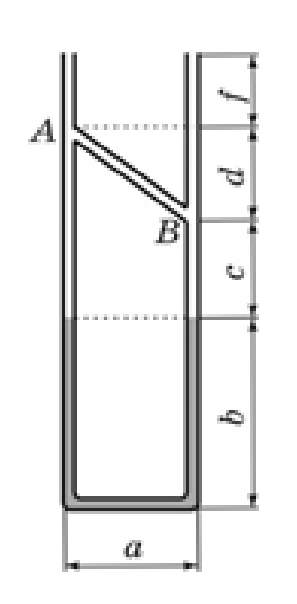
\includegraphics[width=0.5\linewidth]{class10/vuo_2019_85}
			\caption{}
			\label{fig:vuo201985}
		\end{subfigure}
		\begin{subfigure}{.4\textwidth}
			\centering
			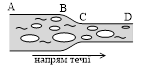
\includegraphics[width=0.5\linewidth]{class10/vuo_2018_83}
			\caption{}
			\label{fig:vuo201883}
		\end{subfigure}
		\begin{subfigure}{.4\textwidth}
			\centering
			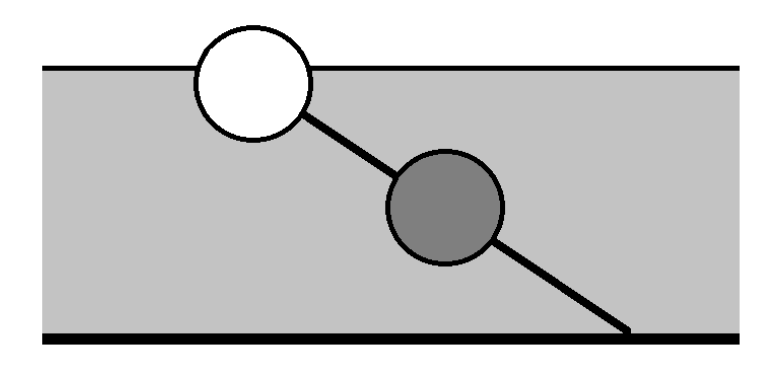
\includegraphics[width=0.5\linewidth]{class10/vuo_2013_85}
			\caption{}
			\label{fig:vuo201385}	
		\end{subfigure}
		\caption{}
	\end{figure}
	
\end{problem}